\documentclass[a4paper]{article}
\usepackage{enumitem}
%% Language and font encodings
\usepackage[english]{babel}
\usepackage[utf8x]{inputenc}
\usepackage[T1]{fontenc}
\usepackage{minted}
\usepackage{float}
\usepackage{multicol}
\usepackage[compatibility=false]{caption}

\usepackage{wrapfig}
%% Sets page size and margins
\usepackage[a4paper,top=2cm,bottom=2cm,left=2.5cm,right=2.5cm,marginparwidth=1.75cm]{geometry}

%% Useful packages
\usepackage{amsmath}
\usepackage{url}

\usepackage{graphicx}
\usepackage[colorinlistoftodos]{todonotes}
\usepackage[colorlinks=true, allcolors=blue]{hyperref}

\title{Native OCaml compiler support on the ESP32 microcontrollers}
\author{Lucas Pluvinage}
\date{}
\setcounter{tocdepth}{2}
\setlength{\parindent}{0cm}
\setlength{\parskip}{1ex plus 0.5ex minus 0.2ex}
\newcommand{\hsp}{\hspace{20pt}}
\newcommand{\HRule}{\rule{\linewidth}{0.5mm}}

\begin{document}

\begin{titlepage}
  \begin{sffamily}
  \begin{center}


    \textsc{\LARGE École Normale Supérieure de Paris}\\[2cm]

    \textsc{\Large Internship report -- M1}\\[1.5cm]

    % Title
    \HRule \\[0.4cm]
    { \huge \bfseries Native OCaml compiler support on the ESP32 microcontrollers\\[0.4cm] }

    \HRule \\[2cm]

    % Author and supervisor
    \begin{minipage}{0.4\textwidth}
      \begin{flushleft} \large
        Lucas \textsc{Pluvinage}\\
      \end{flushleft}
    \end{minipage}
    \begin{minipage}{0.4\textwidth}
      \begin{flushright} \large
        \emph{Advised by } Anil Madhavapeddy, University of Cambridge Computer Laboratory
      \end{flushright}
    \end{minipage}

    \vspace{4cm}
    
    
\includegraphics[width=0.2\columnwidth]{lightbulb.png}
    
    \vfill

    % Bottom of the page
    {\large February 26, 2018 — July 27, 2018}

  \end{center}
  \end{sffamily}
\end{titlepage}

\begin{abstract}
From March to July 2018 I've been doing my research internship with Anil Madhavapeddy in the University of Cambridge Computer Laboratory's \textit{OCaml Labs}. 
This internship was about systems and compilation for micro-controllers, working with the OCaml programming language, 
the Mirage operating system library and ESP32 as the micro-controller target. My goal was to extend and test OCaml capabilities on embedded devices by 
developing a new compilation backend targeting ESP32 processors and porting Mirage operating system unikernel framework to this platform. 
As this has been achieved with success, this internship results in a proof-of-concept for safe and portable programming on a cross-compiled software environment 
targeting constrained devices. In the end I've been able to get an OCaml compilation backend for ESP32 micro-controllers and a fully working Mirage system including network features, and this work will be presented in a talk at ICFP 2018 OCaml Workshop\footnote{\url{https://icfp18.sigplan.org/event/ocaml-2018-papers-ocaml-on-the-esp32-chip-well-typed-lightbulbs-await}}.
I warmly thank Anil Madhavappedy and Gemma Gordon for having me there, as well as the whole OCaml Labs staff and interns with whom 
I had really good times and for some helped me in my project.
\end{abstract}
\tableofcontents
\newpage
\section{Introduction}
\subsection{OCaml}
\begin{wrapfigure}{r}{\columnwidth/4}
	
\includegraphics[width=\columnwidth/4]{ocaml.png}
    \caption{OCaml logo}
\end{wrapfigure}
\paragraph{}
OCaml is a programming language that allows functional, imperative and object-oriented programming styles. The project started 22 years ago and is maintained by 
INRIA (French Institute for Research in Computer Science and Automation). Each system release has a publication which describes the language. For my project, I 
relied on the 4.06 system release \cite{leroy2017ocaml}. OCaml features both a bytecode runtime and native high-performance compilation, uses a garbage 
collector and offers neat features such as a powerful type system, pattern matching, functors (parametric modules) and various optimisations like tail-recursion. 
OCaml Labs has been founded in 2012 by Anil Madhavappedy to promote the usage of OCaml in real world applications. Anil also constributed to \textit{Real World OCaml} 
\cite{minsky2013real} which is a nice reference to learn about the language. OCaml has been derived into another syntax named ReasonML which is developped and 
maintained by Facebook. Here is an example of how OCaml looks:
\begin{minted}{ocaml}
(* Defines a type to represent binary trees. *)
type tree =
  | Leaf
  | Node of int * tree * tree
 
(* Recursive function that computes the sum of values in the tree. *)
let rec sum item =
  match item with
  | Leaf  -> 0
  | Node (value, left, right) -> value + (sum left) + (sum right)
  
(* Create a tree. *)
let myTree =
  Node(
    1,
    Node(2, Node(4, Leaf, Leaf), Node(6, Leaf, Leaf)),
    Node(3, Node(5, Leaf, Leaf), Node(7, Leaf, Leaf))
  )
 
(* Compute the sum of myTree's nodes. *)
let _ = Printf.printf "The sum is %d\n" (sum myTree)
\end{minted}
\paragraph{}
Type features, maturity in the project, a high number of packages trough \href{https://opam.ocaml.org/}{opam} package manager, and an efficient compiler makes OCaml a pretty good subject 
of research considering that we want to port a language for a micro-controller architecture. This makes another step towards OCaml versatility in applications.
\begin{wrapfigure}{r}{0.4\columnwidth}
	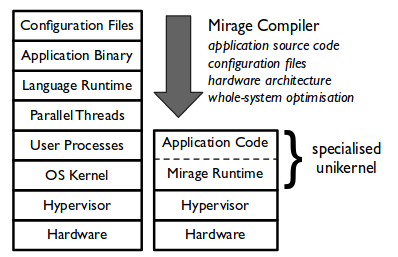
\includegraphics[width=0.4\columnwidth]{unikernel.png}
    \caption{Software stack simplification for specialized applications using Mirage. Taken from \textit{Unikernels: Library Operating Systems for the Cloud}}
\end{wrapfigure}
\subsection{Mirage}
\paragraph{}
Mirage is an operating system unikernel framework written in OCaml first released in 2013 \cite{madhavapeddy2013unikernels}. An unikernel is a single purpose application destined to 
run on bare metal or within a virtualized environment. As a consequence it ships its system dependencies as libraries and don't rely on a traditional operating 
system interface, thus condensing the applicative stack. 
\paragraph{}
The advantages of unikernels in comparison to traditional applications is that unikernels can be:
\begin{itemize}
    \item \textit{faster} as they get rid of the kernel/user separation. By removing context switches, the application can be subject to more efficient optimizations.
    \item \textit{lighter} as the application can ship only useful code. Static analysis and link time optimizations can lead to dead code elimination, 
    this can't be achieved within a traditional operating system.
    \item \textit{safer} as not having an operating system and shipping minimal code greatly reduces the surface of attack of the application. 
    The surface of attack is the set of all weak points of the application. Having a general purpose operating system leads to a broad surface of 
    attack as each functionality can introduce a weak point. By removing all unused functionalities (such as the write feature in a filesystem, 
    remote control features, ..) the unikernel application reduces its surface of attack to code that is actually needed for the application. 
    No more unsecure telnet server that has unintentionally been left on your router OS!
\end{itemize}
Mirage offers the ability to easily build unikernel applications by taking advantage of OCaml features. 
\subsection{ESP32}
\subsubsection{Architecture}
\begin{wrapfigure}{r}{\columnwidth/3}
	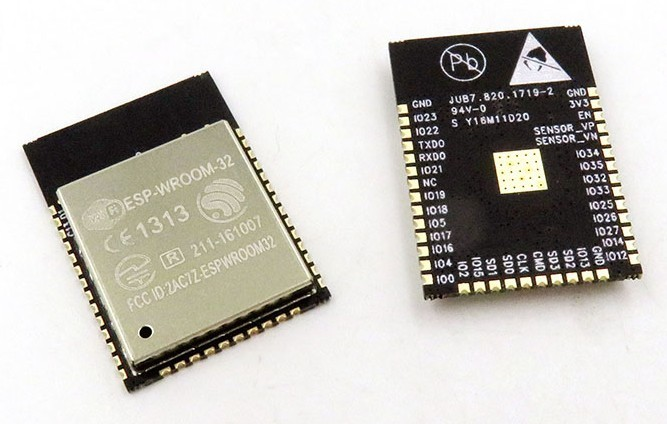
\includegraphics[width=\columnwidth/3]{esp32-wroom-s32-02.jpg}
    \caption{An ESP32 module. Its dimensions are 18x25.5x2.8mm. ESP32 are also sold as development boards.}
\end{wrapfigure}
\paragraph{}
ESP32 is a series of micro-controllers designed by Espressif and released in late 2016. They are designed as low-power, low-cost, 
high-connectivity chips with an aim for embedded applications.  In this section I'll take an overview of the hardware embedded in that chip. The datasheet is available online\footnote{\url{https://www.espressif.com/sites/default/files/documentation/esp32_datasheet_en.pdf}}.
\paragraph{System} The microcontroller relies on a dual-core 240MHz Xtensa LX6 processor along with 520kB of internal RAM and 4MB of flash 
memory, making a really good programming environment for embedded applications (some says that it's overpowered, but we'll talk about power later). 
Xtensa is a series of configurable RISC processors developped by Tensilica which aims for versatility with a customizable instruction set. 
An Xtensa processor is designed by taking the core architecture, adding off-the-shelf features such as floating point support, memory protection, 
exceptions, which are all described in the Xtensa Instruction Set Architecture reference, and designing additional hardware features if needed, 
using the Tensilica Instruction Extension language. The Xtensa LX6 variant has the following specification:
\begin{itemize}[itemsep=0pt,parsep=0pt]
    \item RISC core architecture
    \item 5-stage pipeline
    \item 16/24 bits instruction size
    \item 16 general purpose 32 bits registers named `a0` to `a15`
    \item Windowed registers: the 16 registers are mapped onto 64 physical registers according to a window offset value. 
    When used with special calling conventions this can greatly reduce register spilling.
    \item Interrupt vector
    \item Single-precision floating-point coprocessor
    \item Boolean registers
    \item Digital Signal Processing features
\end{itemize}
If 520K of RAM is not enough, ESP32 supports external SPI-connected RAM and some chips are sold with an additional amount of 4M external RAM. 
Flash size is also configurable, from 1MB to 16MB. 
\paragraph{Low-power} This chip has great focus on low-power features. It's possible to put the whole chip in deep sleep and program an ultra 
low-power coprocessor (ULP) to read sensors, timers, perform light computations and wake the chip up when needed. 
The ULP is a 16-bit, 4 registers processor programmed by writing in a special memory that remains usable in deep sleep (RTC slow memory).
It's also possible to dynamically update the main processor frequency, choosing between 80MHz, 160MHz and 240MHz. According to the datasheet, power consumption at 3.3V usually ranges from 0.1mA to 68mA with spikes up to 0.3A on extensive usage of Wifi/Bluetooth.
\paragraph{Connectivity} ESP32 features an onboard Wifi transceiver and Bluetooth connectivity. Wifi supports modern protocols and encryption types, with hardware acceleration. Moreover it implements a proprietary long range/low bandwidth protocol over Wifi which claims a range of 1 kilometer\footnote{\url{https://blog.hackster.io/long-range-wifi-for-the-esp32-9429ab89f450}}. The Bluetooth controller supports 4.2 Low-Energy (BLE) and classic Bluetooth. During my internship I focused on Wifi networking features and let Bluetooth for future work.
\subsubsection{ESP-IDF and FreeRTOS}
\paragraph{} 
\begin{wrapfigure}{r}{\columnwidth/2}
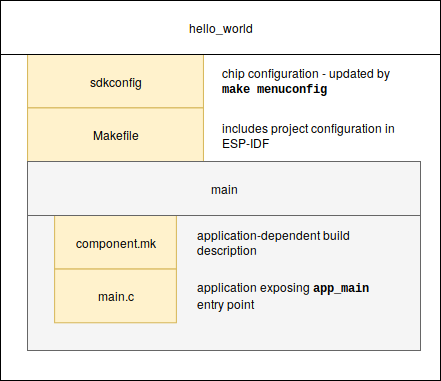
\includegraphics[width=\columnwidth/2]{ESP-IDF.png}
\caption{Directory layout for a project application using ESP-IDF.}
\end{wrapfigure}
Espressif's Iot Development Framework is the best way to program an ESP32 chip as it gives you the low level features through a C API. Wifi drivers are accessible within a simple interface, and even allows you to use high level features such as network sockets trough LwIP. The framework also ships mandatory bootloader code and link scripts that exports hidden internal symbols. Most of the code base is open source and available on Github, but there are still hidden code such as Wifi and Bluetooth internal drivers. 
The ESP32 software layer is based on FreeRTOS which is a preemptive Real-Time Operating System. It provides scheduling for multi-tasking, inter-task communication, timings and synchronisation primitives. This lightweight kernel is used as a foundation for more complex applications. Documentation for this framework is available online\footnote{\url{https://esp-idf.readthedocs.io/en/latest/}}.
\paragraph{} 
It's really hard to build an application without this framework, because it provides hardware drivers as libraries that would be otherwise painful to implement. It might be possible to get rid of the ESP-IDF but it's out of scope for this internship.
I will therefore rely on ESP-IDF as a base for building OCaml applications on ESP32. To build and flash an ESP32 application, it's only needed to have a GCC cross-toolchain (one is provided and maintained by Espressif) and the ESP-IDF repository downloaded somewhere, its location being exposed by \texttt{IDF\_PATH} environment variable. This being set-up, a project consists in a \texttt{sdkconfig} file in a directory, a \texttt{Makefile} that includes ESP-IDF project Makefile, and a component directory containing a configuration makefile to build the component and code.
In a nutshell to have some code running on ESP32, the application component just have to be able to build an Xtensa object file containing an \texttt{app\_main} symbol. This symbol is the entry point of the application, which will be called when the system is initialized. Therefore the hardware boot and low-level system setup is achieved by ESP-IDF code, which has spared me a lot of debugging.
\subsection{Previous work}
\paragraph{}
Previous work has been done on getting OCaml running for ESP32 chips. It has been achieved by Sadiq Jaffer who got a first proof-of-concept of bytecode execution. He explained the process on his blog\footnote{\url{https://toao.com/blog/getting-ocaml-running-on-the-esp32}}, and the experiment has yield some issues which were starting points for my internship.
\paragraph{}
Previous work on cross-compilation with OCaml was done by \href{https://whitequark.org}{whitequark} who designed cross-compilation toolchains for \href{https://github.com/ocaml-cross/opam-cross-android}{Android}, \href{https://github.com/ocaml-cross/opam-cross-ios}{IOS} and \href{https://github.com/ocaml-cross/opam-cross-windows}{Windows}.
\subsection{Internship overview}
Here is a more detailed overview of what I did these 5 months. My work can be found on Github in the \texttt{well-typed-lightbulbs}\footnote{\url{https://github.com/well-typed-lightbulbs/}} organization that I created for the occasion. I also wrote 6 blog posts on my personal website\footnote{\url{https://www.lortex.org/esp32/}}.
\subsubsection{March}
\paragraph{}
As I arrived in the lab, Anil gave me two main endgoals: porting MirageOS unikernel library to ESP32 micro-controllers, and getting a native compilation backend for the OCaml compiler. These two goals seemed fairly independent as Sadiq Jaffer has been able to port the OCaml bytecode runtime on ESP32 architecture. My first thought was that I would be able to port Mirage packages by cross-compiling C code and compiling OCaml code to bytecode. I spent a lot of time discovering Mirage and ESP32 ecosystems that I'll take time to explain further on. I got the opportunity to participate in the MirageOS spring hack retreat in Marrakesh, this was a great way to learn about unikernels, and understand the structure of such a library. 
\subsubsection{April}
\paragraph{}
The OCaml compiler source code is pretty pleasant to read, but severly lacks of documentation. My time was spent reading very old commits from Xavier Leroy and taking the ARM backend as a base for my Xtensa backend. Most of the backend has been built during this month, this was a fun time reading documentation and chasing bugs. 
In the meantime I worked with the opam package manager to package my Mirage port. 
\subsubsection{May}
\paragraph{}
I've got my first unikernel running, it printed Hello every second, with a time stamp shown and a LED blinking. After that some work was done in making this build reproducible. Eventually I've been able to get Wifi networking features and controlling the LCD display. I also developped a semi-automatic porting tool of opam packages.
\subsubsection{June}
\paragraph{}
I focused on porting Mirage libraries in order to get more features available for ESP32. My main work was to get a full TCP/IP stack and a webserver running on the platform. I also worked on build reproducibility and packaging. Another great step was to get dead code elimination which had a great impact on memory usage of applications.
\subsubsection{July}
\paragraph{}
Some optimisations were done on the backend, and I also cleaned up some code. At this stage the goal was to finalize my work by publishing clean packages and setting up reproducible build for sample applications. 

\section{A new OCaml backend}
To run an OCaml program, two choices are available: 
\begin{itemize}[itemsep=0pt,parsep=0pt]
    \item Compile it to bytecode with \textbf{ocamlc} and run it with \textbf{ocamlrun}
    \item Compile it with the native code compiler \textbf{ocamlopt}
\end{itemize}
\paragraph{}
When dealing with a new target, bytecode execution is easier to achieve in comparison to the other.
Therefore my first focus was to run OCaml programs with to the bytecode compilation path. My OCaml backend for ESP32 can be found on Github\footnote{\url{https://github.com/well-typed-lightbulbs/ocaml-esp32/tree/4.06-esp32+lto}}.
\subsection{Bytecode compilation on ESP32}
\begin{wrapfigure}{r}{0.5\columnwidth}
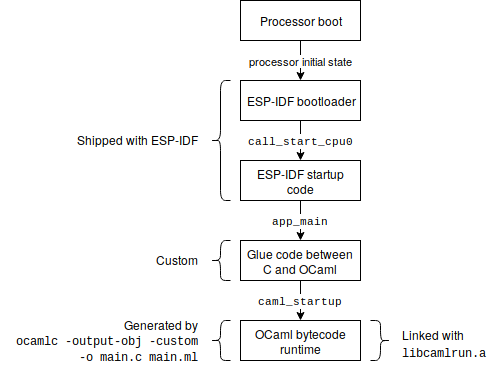
\includegraphics[width=0.5\columnwidth]{Bytecode_comp.png}
\caption{Execution scheme of an OCaml bytecode application on an ESP32 device.}
\end{wrapfigure}
\paragraph{}
One big advantage of bytecode is that it's architecture-independant code. As a consequence, to get OCaml running on a new architecture, the only thing that needs to be achieved is to build the bytecode interpreter library. Once it's available, an OCaml application can be built for ESP32 by compiling it to bytecode, embed it in C and link it with the bytecode interpreter library and ESP-IDF. 
\subsubsection{Compiling \texttt{libcamlrun.a}}
\paragraph{}
\texttt{libcamlrun.a} is the OCaml bytecode interpretation library which embeds a full OCaml runtime for bytecode execution. It's full written in C, and relies on a small subset of \texttt{libc} which enables easy cross-compilation. On ESP32, the GCC cross-toolchain's libc is a Newlib implementation which is designed for memory and size constrained devices. The OCaml 4.06.0 source code has been my starting point in my work on the compiler. 
\paragraph{Configuring the compiler}
Cross-compilation support on OCaml is not very glorious, but it's possible to build an OCaml cross-compiler by downloading the source code and using a parameter in the configure script. The parameter is \texttt{-target}, it is a target triplet (CPU - vendor - system) that corresponds to the desired compilation target. However the target that we want to have \texttt{xtensa-esp32-elf} doesn't exist yet, so the first thing to do was to update the configure script. 
\paragraph{Tweaking parameters}
To support our target, several updates had to be made. 
\begin{itemize}
\item Updating the configuration script to tell OCaml to use the GCC cross-toolchain for ESP32. This is also where some architecture-dependant options are set-up.
\item OCaml is primarily designed for targets that have a decent amount of memory. This is not the case of ESP32 and configuration files have been updated to follow ESP32 memory conditions (520KB of RAM).
\end{itemize}
After that it was possible to get a \texttt{libcamlrun.a} to link with OCaml bytecode and ESP-IDF. This work was introduced by Sadiq Jaffer who was the first to run OCaml code on ESP32. His sample was made of callbacks to C code in order to output text and blink a LED. 


\subsubsection{Personal contribution}
\paragraph{}
That's when I come into play, as some problems remained. The first one was that OCaml's \texttt{Printf} module didn't work. This was fixed by digging into ESP-IDF and OCaml library code. I figured out that OCaml opened file descriptor 1 for output, but at this time ESP-IDF didn't have a proper file descriptor system. In fact ESP-IDF had file descriptor 1 hardcoded to \texttt{/dev/uart1}, a not wired up serial output on the board.
\paragraph{}
The second one is that as the bytecode was loaded in RAM, applications with more modules than a single \texttt{Printf} became too big to fit on a single chip. 520KB of RAM is short, but 4MB of flash should be sufficient for more complex applications. 
My tought was that OCaml bytecode could be read-only and therefore set in flash. Bytecode is embedded in C as 2 arrays of char, one for code and one for data. Setting the code array to \texttt{const} should do the trick, right? Well actually not, it lead to illegal stores. Bytecode is not const for a reason: it's actually rewritten on statup to update instructions if the code is threaded or if endianness differs. 
Hopefully, none of these was actually occuring and the rewrite step was actually trying to rewrite the save value for each bytecode instruction. 
As the bytecode interpreter library did not rewrite bytecode anymore, I've been able to store the OCaml bytecode on flash memory, which spared a lot of space in RAM. 


\subsection{Native compilation support for Xtensa processors}

I got my way up to bytecode execution, but this was too expensive to be a sustainable option in medium to large scale applications. The space and speed improvement offered by native compilation was needed. 

\subsubsection{OCaml compiler hacking}

Adding a new backend architecture in OCaml consists in 
\begin{itemize}
\item \href{https://github.com/well-typed-lightbulbs/ocaml-esp32/tree/4.06-esp32+lto/asmcomp/xtensa}{\texttt{asmcomp/xtensa}}: assembly emission code, made of
    \begin{itemize}[itemsep=0pt,parsep=0pt]
    \item \texttt{proc.ml}: defines registers and calling conventions for OCaml to OCaml and OCaml to C.
    \item \texttt{arch.ml}: gives word size, endianness and addressing modes.
    \item \texttt{emit.mlp}: assembly emitter. This is the core of the native backend, and consists in a \href{https://github.com/well-typed-lightbulbs/ocaml-esp32/blob/4.06-esp32+lto/asmcomp/xtensa/emit.mlp\#L336}{large pattern matching} of the last intermediate representation variant, which given instructions and locations (registers, stack memory) generates assembly instructions. This is a preprocessed file with features a more readable assembly generation code. 
    \item \texttt{selection.ml}: instruction selection from Cmm to the last intermediate representation.
    \item \texttt{CSE.ml}: common subexpression elimination, no architecture-specific work has been done there.
    \item \texttt{reload.ml}: instruction reloading, no architecture-specific work has been done there.
    \item \texttt{scheduling.ml}: it's possible to input instruction timings in order to perform more precise scheduling.
    \end{itemize}
\item \texttt{asmrun}: \href{https://github.com/well-typed-lightbulbs/ocaml-esp32/blob/4.06-esp32+lto/asmrun/xtensa.S}{\texttt{xtensa.S}} contains assembly code that makes the interface between code emitted by the OCaml compiler and the OCaml runtime which is written in C.
\end{itemize}
\paragraph{Example}
This code section is assembly emission for a 3-way branching, with different branches if the register is less than, equal, or greater to 1.
\begin{minted}{ocaml}
| Lcondbranch3(br1, br2, br3) -> 
  begin match br1 with
    | None -> ()
    | Some lbl -> `blti	{emit_reg i.arg.(0)}, 1, {emit_label lbl}\n`
  end;
  begin match br2 with
    | None -> ()
    | Some lbl -> `beqi	{emit_reg i.arg.(0)}, 1, {emit_label lbl}\n`
  end;
  begin match br3 with
    | None -> ()
    | Some lbl -> `bgei	{emit_reg i.arg.(0)}, 2, {emit_label lbl}\n`
  end;
\end{minted}
\paragraph{Compiling a cross-compiler}
The first pre-requisite to compile a cross-compiler is that it's mandatory to build it with the same OCaml version. Moreover natural integer size must be the same between host and target, I therefore used \texttt{ocaml-4.06.0+32bit} version as a base compiler. 
A standard make world tries to build target executables which is not possible in my case. I added a \textbf{world-cross} compilation target that address this issue by compiling only what's needed (ocamlc, ocamlopt, libraries, ocamlmklib). I also had to turn off bootstrapping features. When everything was set up, compiling the compiler would take between one and two minutes.

\subsubsection{Xtensa backend}
OCaml's last intermediate language is not documented, so I reviewed ARM backend to understand what was going on. Xtensa ISA has been my main tool to write the code emitter. I also used gcc and objdump to see how some operations were compiled. Most operations were easy to emit but Xtensa have some specialites that had to be taken into account. My main resource for native compilation was the Xtensa Instruction Set Architecture\footnote{\url{https://0x04.net/~mwk/doc/xtensa.pdf}} and the ESP32 datasheet to figure out which options were enabled.


\paragraph{Register windowing}
At any time a window of 16 registers is visible, and this window can be rotated back and forth of 4, 8 or 12 registers on function call and return. Xtensa ships 64 physical registers, this acts as a highly efficient stack and can yield better performances than 16 fixed registers while keeping instruction register addressing on 4 bits. Register windowing is implemented by:
\begin{itemize}
    \item having more physical registers (64) than visible registers (16)
    \item instructions to rotate the window:
    \begin{itemize}
        \item CALLn label: prepare rotation by N registers by setting the two high bits of the return address according to N and writing to a special register, and jump to specified address (offset).
        \item CALLXn register: same as CALLn but jumps to the address specified in register.
        \item ENTRY n: rotates register window according to the value of the special register and allocates n bytes by updating the stack pointer.
        \item RETW: rotates the window back by an amount determined by the two high bits of the return address that have been previously set up by CALL or CALLX. Then jumps on the concatenation of the 2 high bits of the program counter and the 30 low bits of the return address. Therefore caller and callee must reside in the same 1GB section of memory. This can be assumed on ESP32. 
    \end{itemize}
    \item Calling conventions is what holds everything up. As the rotation is between 4 and 12, there are always a positive number of registers in common between the caller and the callee. This is how parameters and return values are passed. With CALLn, n registers are saved and 16-n registers are in common. Counting the return address and the stack pointer, that makes it 2, 6 or 10 registers that can be transmitted. The \textbf{main} question remains: what happens when the window cycles ? It overflows, as registers are already used, they must be spilled on the stack where the function that owns these registers will be able to find them back. As a consequence the ABI is not a standard one: at each function call there is room kept in case of spilling.
\paragraph{}
Spilling is automatically managed by two exceptions: window overflow and window underflow. Window overflow occurs when a read or write is done on a 4-registers group that is already marked as used. Window underflow occurs when returning to a function that got its registers spilled on the stack.
\end{itemize}

\paragraph{Register windowing in OCaml}
As I started to work on function calls in the backend I found out that windowed registers were not supported. The compiler assumes that caller's and callee's results registers are the same, but this is not the case for windowed registers. I had a choice to make: use the tricky windowed registers calling convention for OCaml compilation along with some compiler hacking to support that, or use flat registers in OCaml mixed with windowed registers in C. I felt that the latter option would be easier to work with, and that's what I chose to implement. As a consequence I had to develop non standard interfaces between windowed and flat calling conventions. 

\paragraph{Negative offset load}
The fastest way to load a value into memory is to use the L32I instruction. It's a load from a register address with a non-negative immediate -- multiple of 4 -- offset with a range from 0 to 1020. This instruction is mostly used for stack and heap access. However there is a case where a negative offset has to be used, and that's because of the internal representation of OCaml blocks. Blocks are OCaml values allocated on the heap, represented by the address of the data segment of the block. Block header is accessed by accessing the 32 bit value at data address minus 4 bytes. 
That is a negative offset, hopefully the shorter range L32E existed for windowed registers features and is useful in our case. 

\paragraph{Conditionals}
To achieve conditionals two sets of instructions are available, but they do not cover every kind of comparisons:
\begin{itemize}[itemsep=0pt,parsep=0pt]
    \item Conditional move: one register $= 0, \neq 0, < 0, \geq 0$.
    \item Cond. branch: two registers or a register and an immediate value, signed or unsigned $=, \neq, <, \geq$.
\end{itemize}
It's possible to achieve every kind of conditional branch by using simple transformations:
\begin{itemize}[itemsep=0pt,parsep=0pt]
\item $r1 > r2 \iff r2 < r1$ 
\item $r1 \leq r2 \iff r2 \leq r1$
\item $r1 > n \iff r1 \geq n+1$ 
\item $r1 \leq n \iff r1 < n+1$
\end{itemize}
\paragraph{Exception handling with windowed registers}
In OCaml, a try-with block is implemented by pushing data on the stack when entering the block, popping it when leaving, and using the data when an exception is raised. The \textit{trap pointer} is a special register that holds the innest try-with block data. Each try-with block holds a pointer to its exception handler and a pointer to the outer try-with block data, with the last exception block pointing to the default handler that prints a \textbf{Uncaught exception message}. 
Special work has been done on exception handling as windowed registers makes it a bit trickier. When an exception is thrown, either the window needs to be rotated back to the correct level in the catch handler, or make sure every register is spilled before continuing. 
In OCaml-only code, there is nothing to do as I use a flat calling convention with no register windowing, so a standard exception procedure can be used. However raising an OCaml exception from C as done by \href{https://github.com/well-typed-lightbulbs/ocaml-esp32/blob/4.06-esp32/asmrun/xtensa.S\#L332}{\texttt{caml\_raise\_exception}} needs to spill every windowed register before jumping in the exception handler. This is done using a dummy syscall.  

\subsection{Cross-compiling for ESP32 microcontrollers}
\subsubsection{Integration with OCaml compilation}
\paragraph{}
The prerequisite for ESP32 cross-compilation are to have a GCC cross-toolchain, the ESP-IDF and an OCaml cross-compiler with my backend implemented. The compilation flow is the following:
\begin{itemize}[itemsep=0pt,parsep=0pt]
	\item Write \texttt{.ml} files.
    \item Use \texttt{ocaml -output-complete-obj} to create a library which exposes OCaml entry point \texttt{caml\_startup}. 
    \item Glue code written in C that calls \texttt{caml\_startup} and exposes \texttt{app\_main}.
	\item Configuration and linking step with ESP-IDF.
	\item Flash the chip.
\end{itemize}


\subsubsection{Integration with build systems}
\paragraph{}
There are a lot of build systems used by OCaml packages that have more or less support for cross-compilation. I had to learn about them in order to port the packages I needed to the ESP32 platform.
\begin{itemize}
    \item Dune (formerly Jbuilder): this is probably the most popular build system used to build Mirage packages. It provides cross-compilation support trough the \texttt{-x esp32} option. It has support for preprocessors and requires in most cases no other modification to cross-build the package. When building with \texttt{-x target}, it looks for target packages in the \texttt{target-sysroot/lib} subdirectory of the current opam switch, and builds with \texttt{target-sysroot/bin} binaries. 
    \item OCamlbuild/OASIS: used for some packages, it uses \texttt{ocamlfind} to figure out where cross-compiled packages and the cross-compilation toolchain are located. Both expose a \texttt{-toolchain} option that is transmitted to \texttt{ocamlfind} which is configured by a file written when the toolchain is installed. In order to be compatible with \texttt{jbuilder}, the \texttt{ocamlfind} configuration file points to \texttt{esp32-sysroot} subdirectory for binaries and packages. 
    \item Makefile: often handmade for old packages, these are the hardest to cross-compile as tweaking is mandatory. When they use \texttt{ocamlfind}, \texttt{env OCAMLFINDTOOLCHAIN=esp32 make} can be sufficient to cross-compile files. However sometimes compiler and feature discovery can be completely hardcoded, letting me with no choice but to rewrite the Makefile or setting up the package with a modern build system.
\end{itemize}

\subsection{How to port a package for a new architecture}
\subsubsection{The opam package manager}
\paragraph{}
Even if there are a lot of build systems to use, at least OCaml is provided with a single package manager that everyone use. Opam is a source-based package manager that supports multiple compilation installations, named as switches. Each switch relies on a chosen version of an OCaml compiler and has its own set of packages. Its main repository\footnote{\url{https://github.com/ocaml/opam-repository}} is managed by OCaml Labs but it's possible to add custom repositories, as I've done for ESP32.

\subsubsection{Ad-hoc support for cross-compilation}
\paragraph{}
It's easy to think that cross-compilation is just a matter of installing a switch with the cross-compiler as a base compiler, but it's not the case as it's almost mandatory to have an host compiler to build packages. It's because of preprocessors. Preprocessors is pieces of code written in OCaml that allow OCaml code to extend its syntax. These are used to lower the amount of code to write by generating boilerplate that no one wants to write. A good example for this is the \texttt{cstruct} rewriter that allows to use structures from C in OCaml. 
For example, this code describes an Ethernet II header data structure:
\begin{minted}{ocaml}
[%%cstruct
type ethernet = {
  dst: uint8_t [@len 6];
  src: uint8_t [@len 6];
  ethertype: uint16_t;
} [@@big_endian]]
\end{minted}
The \texttt{cstruct} preprocessor automatically generates the following signature with the corresponding implementation:
\begin{minted}{ocaml}
val sizeof_ethernet : int
val get_ethernet_dst : Cstruct.t -> Cstruct.t
val copy_ethernet_dst : Cstruct.t -> string
val set_ethernet_dst : string -> int -> Cstruct.t -> unit
val blit_ethernet_dst : Cstruct.t -> int -> Cstruct.t -> unit
val get_ethernet_src : Cstruct.t -> Cstruct.t
val copy_ethernet_src : Cstruct.t -> string
val set_ethernet_src : string -> int -> Cstruct.t -> unit
val blit_ethernet_src : Cstruct.t -> int -> Cstruct.t -> unit
val get_ethernet_ethertype : Cstruct.t -> Cstruct.uint16
val set_ethernet_ethertype : Cstruct.t -> Cstruct.uint16 -> unit
val hexdump_ethernet_to_buffer : Buffer.t -> Cstruct.t -> unit
val hexdump_ethernet : Cstruct.t -> unit
\end{minted}
\paragraph{}
Opam doesn't know about cross-compilation, so there is no standard to set up such an environment. I've been inspired by \texttt{whitequark} to create an \texttt{opam-cross-esp32}\footnote{\url{https://www.github.com/well-typed-lightbulbs/opam-cross-esp32}} repository which contains all the packages I ported for my cross-compilation environment. As in \texttt{opam-cross-windows}, \texttt{opam-cross-android} and \texttt{opam-cross-ios}, my repository contains an \texttt{ocaml-esp32} package which installs the cross-compilation toolchain for ESP32 in the \texttt{esp32-sysroot} subdirectory of the current switch. It also configures \texttt{ocamlfind} to properly point to cross-binaries and packages when used with the \texttt{-toolchain esp32} option. Packages are then installed in the \texttt{esp32-sysroot/lib} subdirectory.
\paragraph{}
\texttt{ocaml-esp32} has only two dependencies. The first is \texttt{ocamlfind} in order to be able to install the configuration file. The second one is \texttt{gcc-toolchain-esp32} which is a package that installs the cross-toolchain for ESP32 in the switch and makes it available in the \texttt{PATH}.
\paragraph{} In order to avoid name clash, every cross-compiled package for ESP32 has an \texttt{-esp32} suffix. For packages that already have \texttt{-esp32} as a suffix -- such as system-specific Mirage implementations -- it's replaced by \texttt{-impl-esp32} for aesthetic purpose. 
\subsubsection{Porting packages}
\paragraph{} 
Porting Dune packages is easy because of the \texttt{-x esp32} option that automatically generates an installation file for the correct prefix, which is \texttt{esp32-sysroot/lib}. Manual work remains when the code includes non portable C. For other packages installation is more or less easy, with sometimes having to specify in which directory the package should be installed.
\paragraph{}
I've developed an automatic port tool -- named \texttt{opam-ezport}\footnote{\url{https://github.com/TheLortex/opam-ezport}} -- which aims to semi-automatically port packages to a platform by importing the opam definition, adding an \texttt{-esp32} suffix and adding \texttt{-x esp32} when a dune build system is recognized, and doing this recursively for dependencies. It also imports packages from other build systems but does nothing to it beside indicating that manual work has to be done.

\section{Unikernels for embedded applications}
As I got a native compilation backend, a part of Mirage unikernel library has been ported to ESP32 as a base for real world applications.
\subsection{Unikernels and Mirage}
\subsubsection{What is an unikernel ?}
\paragraph{}
\begin{wrapfigure}{l}{0.4\columnwidth}
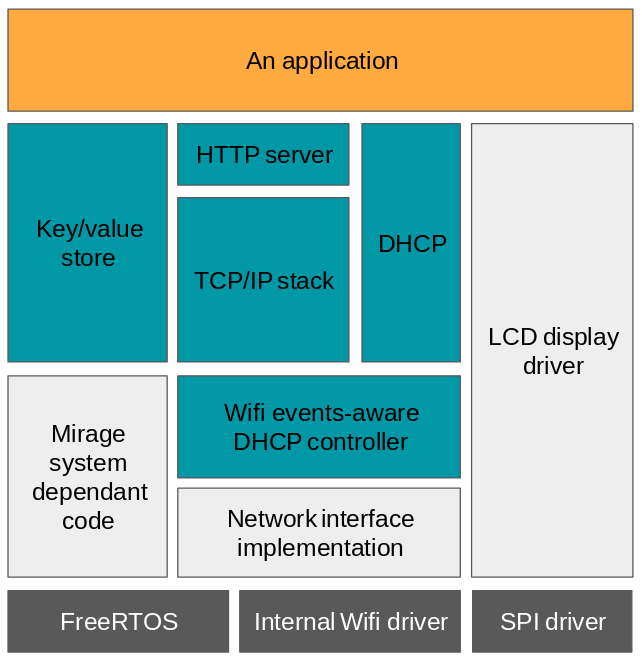
\includegraphics[width=0.4\columnwidth]{app.png}
\caption{Full unikernel stack sample for ESP32. Blue is full OCaml code. Grey is my C/OCaml interface implementation. Black is ESP-IDF, written in C.}
\end{wrapfigure}
A traditional application relies on an operating system to run. A part of the operating system is the kernel which provides system features trough system calls which makes the interface between hardware and applications. When the application needs a system feature, such as input/output, it calls the kernel and cause a context switch which put the processor from user into privileged mode while the kernel executes I/O operations. Unikernels get rid of the user/kernel separation. The application is directly linked to system features and runs in priviledged mode. 
\paragraph{}
This allows an application to be shipped with only the code it needs. Using specialized system features as a library instead of general purpose operating system has several advantages. It reduces code size thanks to dead code eliminations, increase speed by getting rid of kernel context switches and thus allowing more aggressive optimizations, and increases safety by reducing the code base size, decreasing the surface of attack of a specialized application and opening the door to formal proving of system features. Unikernels allow the deployment of lightweight single-purpose virtual machines, which are in theory more efficient than a single-purpose application on a general purpose virtual machine. Typical unikernel applications include DNS, DHCP and HTTPS\cite{mehnert2014transport} servers and that's what I wanted to get running during my internship.
\subsubsection{Mirage ecosystem}
\paragraph{}
The Mirage ecosystem is a framework that builds unikernel applications written in OCaml. It can target unix operating systems, and virtualized environments such as Xen \cite{barham2003xen} and ukvm. Mirage is composed of a command line interface and a library made of dozens of opam packages\footnote{\url{https://github.com/mirage}}. 

\paragraph{Mirage library}
Mirage gives module signatures and type definitions to define the system features that the library wants to offer. 
These can be found in the \texttt{mirage-types}\footnote{\url{https://github.com/mirage/mirage/blob/master/types/mirage\_types.ml}} 
package and dependencies. For each feature there is a package defining types for this feature. 
For example \texttt{mirage-random} defines a \textbf{Mirage\_random.S} signature:
\begin{minted}{ocaml}
module type S = sig
  (** The type for memory buffer. *)
  type buffer                         
   (** The state of the generator. *)
  type g                             
  (** [generate ~g n] generates a random buffer of length [n] using [g]. *)
  val generate: ?g:g -> int -> buffer 
end
\end{minted}
\paragraph{}
These module types serve as a base for more complex Mirage modules, such as a web server. Module implementations 
are either portable or specialized in different packages. For example Mirage protocols signatures are implemented 
by \href{https://github.com/mirage/mirage-tcpip}{\texttt{tcpip}} in a portable way, relying on a \texttt{Mirage\_net.S} 
module implementation which is not portable. As a consequence the \texttt{Mirage\_net.S} signature has a different 
implementation whether it's targeting Unix\footnote{\href{https://github.com/mirage/mirage-net-unix}{mirage-net-unix}} or Xen\footnote{\href{https://github.com/mirage/mirage-net-xen}{mirage-net-xen}}. 
A goal was to identify system-specific implementations and add my own for ESP32 target.
\paragraph{CLI}
\begin{wrapfigure}{r}{0.4\columnwidth}
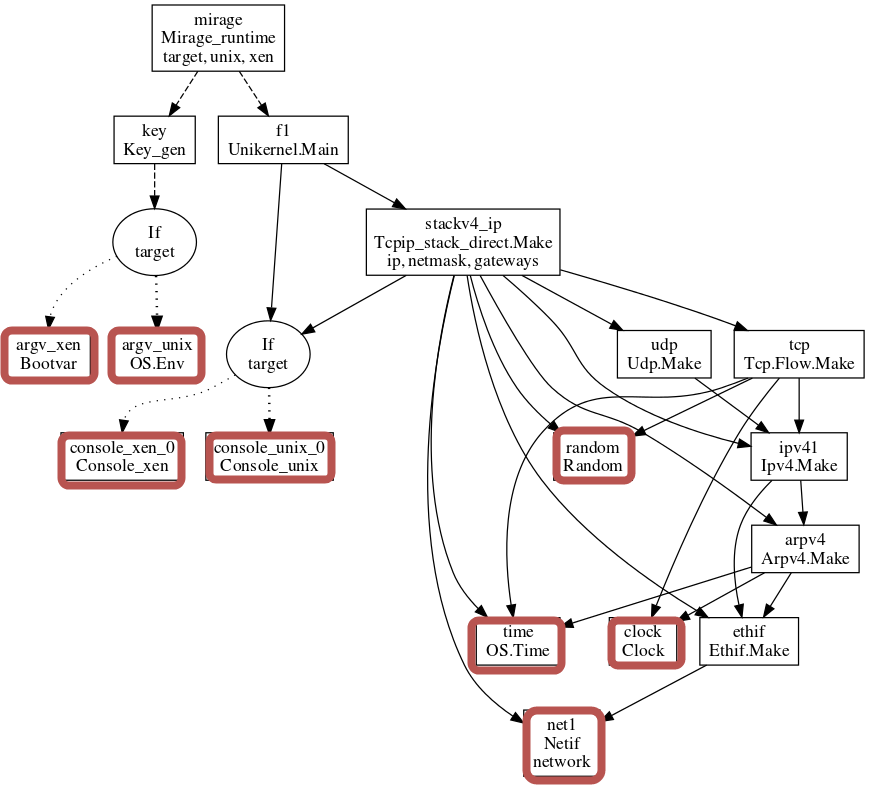
\includegraphics[width=0.4\columnwidth]{mirage_app.png}
\caption{Module dependency tree of an unikernel requesting the network stack. In red are the system-dependent features.}
\end{wrapfigure}
Mirage is shipped with a \texttt{mirage} executable which is used to configure and build applications. 
The configuration command is \texttt{mirage config -t <target>} that prepares code and dependencies for 
the chosen target according to the unikernel configuration file \texttt{config.ml}. 
The configuration file specifies which features are used. It also allows to input configuration or runtime parameters, 
these are named \textbf{keys}. Keys in Mirage can be used to choose between two implementations at configuration time, 
or specify a listening port for a server. When \texttt{mirage config} is used, it resolves module dependencies 
for the chosen target, writes package dependencies and generates the startup file which consists in initializing 
requested features before calling the unikernel entry point with the features as parameters.
\subsubsection{Mirage as a functor library}
\paragraph{}
OCaml modules hide implementation behind a signature, which defines types and functions that the module 
makes available. These are useful to separate features into specific namespaces and is the entry point 
to generalization. Module signature allows efficient separation between what is needed for the implementation 
and what is available to the user. Here is an example of an OCaml module and its implementation. 
You can note that the \texttt{message} variable is not externally available.

\begin{figure}[!h]
 \begin{minipage}{0.5\textwidth}
  \centering
  \begin{minted}{ocaml}
module type Hello_type =
sig
  val hello : unit -> unit
end
  \end{minted}
  \caption*{Module signature example}
 \end{minipage}
 \begin{minipage}{0.5\textwidth}
  \centering
  \begin{minted}{ocaml}
module Hello : Hello_type =
struct
  let message = "Hello"
  let hello () = print_endline message
end
  \end{minted}
  \caption*{A module implementing the \texttt{Hello\_type} signature.}
 \end{minipage}
 \caption{Syntax for OCaml modules and signatures}
\end{figure}

\paragraph{}
Functors are modules parameterized by other modules. They allow the design of abstractions and is a good way to increase 
code reusability. For example sets in OCaml are implemented as the \texttt{Set.Make} functor that takes an \texttt{OrderedType} 
module argument. Implementation for sets is therefore abstracted. The drawback is that \texttt{Set.Make} needs to be used for 
every needed set type. A functor can also be constrained by a signature.
\begin{figure}[!h]
 \begin{minipage}{0.5\textwidth}
  \centering
  \begin{minted}{ocaml}
module Hello_twice 
  (H : Hello_type) : Hello_type =
struct
  let hello () =  H.hello (); 
                  H.hello ()
end
  \end{minted}
  \caption*{Functor that takes a module with a hello function and creates a hello function calling  the module's hello twice.}
 \end{minipage}
 \hspace{0.05\textwidth}
 \begin{minipage}{0.45\textwidth}
  \centering
  \begin{minted}{ocaml}
module Hello : Hello_type =
struct
  let hello () = print_endline "¡Hola!"
end
  \end{minted}
  \caption*{Another module implementing \texttt{Hello\_type}.}
 \end{minipage}
 \begin{center}
  \begin{minted}{ocaml}
module H2 = Hello_twice(Hello)
module H3 = Hello_twice(Hello_in_spanish)
module H4 = Hello_twice(Hello_twice(Hello))
let _ = H2.hello (); 
        H3.hello (); 
        H4.hello ()
  \end{minted}
 \caption*{Instanciating modules and calling its functions. Executing this code will print "Hello" twice, "¡Hola!" twice and "Hello" four times}
 \end{center}
 \caption{Functor syntax in OCaml, with a little example. }
\end{figure}

\paragraph{}
Mirage is basically a big set of functors describing portable features relying on a small set of system-dependant modules. 
These functors are plugged together by the \texttt{Functoria} library, which allows configure-time modularity.

\subsection{Mirage system-dependent code}
\paragraph{}
Mirage rely on a very small amount of system-dependent code. Every Mirage target implements an \texttt{OS} module containing the basic features a portable application needs. System-dependent modules used for other purposes such as networking are contained in other packages, but we'll take a look at some of these later. 

\subsubsection{Lightweight threads}
\paragraph{}
Mirage unikernels and libraries are designed as single-process concurrent applications. Concurrency is 
achieved trough cooperative scheduling by extensively using the Lwt (lightweight threads) library introduced in 2008 \cite{vouillon2008lwt}. Instead of relying on a preemptive scheduler that randomly switches between threads according to timer interruptions, Mirage relies on a cooperative model. Whereas threads in a preemptive model doesn't have to do anything, cooperative threads are in charge of calling the scheduler back when their work is done, waiting for input/output or sleeping for a given duration. These instants are \textit{cooperation points}, where the scheduler takes control before jumping to the next task to run.
\paragraph{}
A Lwt thread returning a value of type \texttt{'a} has type \texttt{'a Lwt.t}. Threads can be created and composed respectively with \texttt{return : 'a -> 'a Lwt.t} and \texttt{bind : 'a Lwt.t -> ('a -> 'b Lwt.t) -> 'b Lwt.t}. This actually describes a monad. Lwt features includes synchronization, waiting for events, sleeping threads, concurrent execution (\texttt{join : unit Lwt.t list -> unit Lwt.t} creates a thread that waits for
a list of threads to be executed).
\paragraph{}
To make all of this useful, a single function needs to be implemented: \texttt{run : unit Lwt.t -> unit}. 
This a rather central system-dependent part that I had to implement in the \href{https://github.com/well-typed-lightbulbs/mirage-impl-esp32/blob/master/lib/main.ml}{\texttt{OS.Main}} submodule. In my first version threads could only wait for timer events. This was implemented\footnote{\url{https://github.com/well-typed-lightbulbs/mirage-impl-esp32/blob/master/lib/time.ml}} using a priority queue as an efficient way to look up for the next thread to wake. 
\subsubsection{Time}
\paragraph{}
The \texttt{OS.Time} module is essential for scheduling features and allows thread to sleep for a specified duration. It exposes a monotonic clock with microsecond precision. 
\subsubsection{Event system}
\paragraph{}
As I developed networking features I was in need for a fine-grained way to wait for network events, and events in general. My main inspiration -- solo5 -- actually relies on an all-or-nothing event system, so I had to design it on my own. The goal was to support ESP32 wifi networking events which consists in reacting to wifi startup, connection, disconnection, frame received for access point or station mode. Event features are available in the \href{https://github.com/well-typed-lightbulbs/mirage-impl-esp32/blob/master/lib/event.ml}{\texttt{OS.Event}} module. 
The event system makes use of the \texttt{Lwt\_condition} feature for scheduler to thread notification and the FreeRTOS' event group\footnote{\url{https://www.freertos.org/FreeRTOS-Event-Groups.html}} feature for system to scheduler notifications. 

\subsection{Using functors to build modular code: a wifi library story}
\paragraph{}
My end goal after getting some basic Mirage applications was to take advantage of ESP32's wifi features. ESP-IDF provides a wifi driver and a network stack thanks to lwIP implementation. My goal was to take advantage of the Mirage TCP/IP network stack written in OCaml instead of lwIP. This consisted in writing an ESP32-specific network interface module and building the stack on top of it. 

\subsubsection{Network abstractions in Mirage}
\paragraph{}
Networking features in Mirage are separated in a few packages: \href{https://github.com/mirage/mirage-net}{\texttt{mirage-net}} gives the module signature for a network interface, \href{https://github.com/mirage/mirage-protocols}{\texttt{mirage-protocols}} gives module signatures for Ethernet, ARP, IP, TCP, UDP and ICMP and \href{https://github.com/mirage/mirage-stack}{\texttt{mirage-stack}} gives the module signature for a TCP/IPV4 stack. The \href{https://github.com/mirage/mirage-tcpip}{\texttt{tcpip}} package contains the protocols and stack implementation. The stack module implementation is functor-based which makes it easy to plug in a custom network interface to have the whole stack running.
\subsubsection{Building a TCPIP stack on ESP32}
\begin{wrapfigure}{r}{0.3\columnwidth}
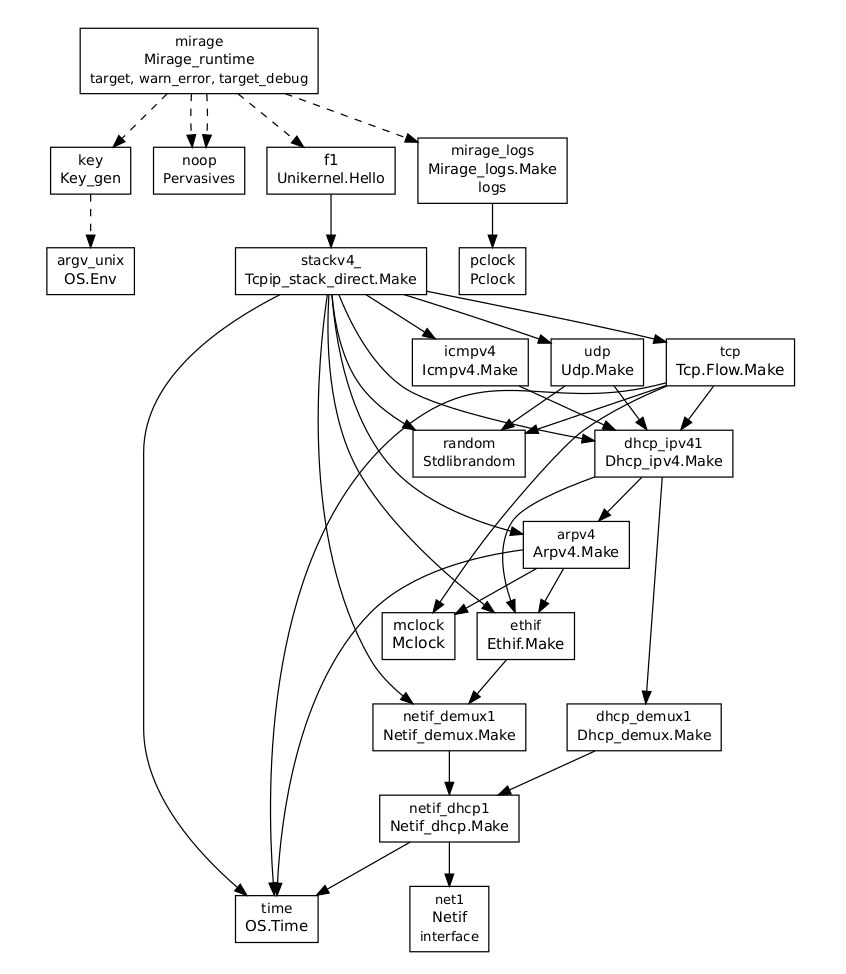
\includegraphics[width=0.3\columnwidth]{unik.png}
\caption{Module dependency tree for a dynamic IP unikernel.}
\end{wrapfigure}
\paragraph{}
Wifi configuration is done in C, using ESP-IDF's driver \footnote{\url{https://esp-idf.readthedocs.io/en/v3.1-rc1/api-reference/wifi/esp_wifi.html}}. The chip has a transceiver, which makes it possible to setup an access point, a station, or both at the same time. When the access point mode is enabled, it supports up to 4 connected devices. My networking code is separated in two packages: \href{https://github.com/well-typed-lightbulbs/wifi-esp32}{\texttt{wifi-esp32}} for general wifi bindings and \href{https://github.com/well-typed-lightbulbs/mirage-net-impl-esp32}{\texttt{mirage-net-impl-esp32}} for the Mirage Wifi network interface module, complying with \texttt{mirage-net} signature. 
\paragraph{}
Whereas Wifi setup is made easy by ESP-IDF, it's not the case of building a custom stack on top of it. Everything is made for lwIP so I had to seek between the Wifi driver and lwIP, looking for how to receive and send frames. Internal driver functions are exposed in \href{https://github.com/espressif/esp-idf/blob/master/components/esp32/include/esp_wifi_internal.h}{\texttt{esp\_wifi\_internal.h}}. This file allow to send and received data frames which is what is needed for a network interface. Sending a data frame is done with \texttt{esp\_wifi\_internal\_tx} and reception callback is set up with \texttt{esp\_wifi\_internal\_reg\_rxcb}.
The reception callback makes the interface between C and OCaml wifi driver, storing pending frames and using the event system to notify upper layers. 

\subsubsection{Integrating DHCP features}
\paragraph{}
For most Mirage applications, a static IP allocated on unikernel startup is sufficient. Therefore the default setup model for DHCP network stacks is:
\begin{itemize}[itemsep=0pt,parsep=0pt]
\item Initialize network interface.
\item Use network interface to get a DHCP lease. Once got, stop using the network interface.
\item Initialize the stack using the obtained lease.
\item Start the main network loop using the network interface. 
\item Start the unikernel application.
\end{itemize}
The problem is that wifi configuration is actually done on the last step, with the possibility to dynamically update wifi settings while keeping the stack running. Wifi settings include mode (station, access point, or both), ssid, password, authentication protocol. To get a DHCP lease, we need the wifi to be configured, therefore leading to a chicken an egg situation. I solved this by making the DHCP process asynchronous. \href{https://github.com/well-typed-lightbulbs/netif-dhcp-esp32}{\texttt{netif-dhcp-esp32}} contains a set of functors that takes a network interface module in input and implements DHCP logic to output a DHCP stream and a network interface connected to upper layers. This layer looks for DHCP packets and transmit them to the DHCP client while transmitting the remaining packets to upper layers.



\section{Conclusion}
\subsection{Issues encountered}
\paragraph{}
The main issue remained that ESP32 fall short in memory when used with OCaml. For simple applications I've been able to reduce memory footprint enough to be able to run it on a 520KB chip, but as I start to use network features the 4MB version is mandatory. Memory optimizations we done in code generation and by porting a dead-code elimination patch. 
\paragraph{}
Cross-compilation support in OCaml was another tale, and I had to use various mysterious hacks to get everything working fine together, even if I haven't mentioned them all in my report. Cross-compilation support should be an important issue in a language ecosystem design and this internship gave me insights on that matter.
\subsection{What remains to do}
\paragraph{}
During this internship I personally felt like some work could be done on the OCaml programming language. The ReasonML syntax appealed to me like a viable option for OCaml development. I also read about modular implicits \cite{white2015modular} that would be a way to solve the issue of function overloading in OCaml. 
\paragraph{}
This work opened a large door for systems development on embedded devices. Adding a new language for a platform is always a nice thing to have, as it brings its whole ecosystem with it. Only a small set of features have been explored, thus remains not implemented Mirage and ESP32 features. It might be interesting to create module abstractions for concrete features such as sensors. This could lead to meta-programming over embedded devices. 
ESP32 features that have not been explored yet include:
\begin{itemize}[itemsep=0pt,parsep=0pt]
\item Ultra-low power processor
\item Crypto-acceleration
\item Bluetooth
\item Sensors I/O (PWM, I2C, SPI, DAC)
\end{itemize}
\paragraph{}
Along with features, build reproducibility and memory optimization are important subjects for cross-compilation on constrained devices. I feel like there remains plenty of work to do in order to get stable builds that doesn't run out of memory. For example something I missed was to get dynamic memory profiling and accurate estimations of how much memory an application will use. 

\subsection{What I have achieved}
\paragraph{}
During this internship I've been able to build native code backend for the OCaml compiler which could potentially go upstream. This backend is efficient enough to be able to run complex applications in such a limited memory environment. This naturally lead to the port of Mirage features from cooperative threads to a TPC/IP stack with TLS support. In the meantime I've been able to create OCaml bindings for Wifi and LCD display. I've been able to create and show live demonstrations of these features in the lab. Samples are available on Github as Docker images\footnote{\url{https://github.com/well-typed-lightbulbs/esp32-docker-samples}} and as plain unikernel code\footnote{\url{https://github.com/well-typed-lightbulbs/mirage-esp32-samples}}.
\paragraph{}
I also ported a compiler patch in order to get cross-module dead-code elimination, which yields a 30\% to 50\% code size reduction for Mirage applications. The compiler was also patched to separate read-write and read-only data in the last intermediate representation.
\paragraph{}
This internship gave me great insights on systems and compilation point of views while teaching me that a lot remains to do.


\bibliography{main}
\bibliographystyle{plain}
\end{document}
